\documentclass[letterpaper,superscriptaddress,showkeys,longbibliography]{revtex4-1}\usepackage{graphicx, color}
%% maxwidth is the original width if it is less than linewidth
%% otherwise use linewidth (to make sure the graphics do not exceed the margin)
\makeatletter
\def\maxwidth{ %
  \ifdim\Gin@nat@width>\linewidth
    \linewidth
  \else
    \Gin@nat@width
  \fi
}
\makeatother

\IfFileExists{upquote.sty}{\usepackage{upquote}}{}
\definecolor{fgcolor}{rgb}{0.2, 0.2, 0.2}
\newcommand{\hlnumber}[1]{\textcolor[rgb]{0,0,0}{#1}}%
\newcommand{\hlfunctioncall}[1]{\textcolor[rgb]{0.501960784313725,0,0.329411764705882}{\textbf{#1}}}%
\newcommand{\hlstring}[1]{\textcolor[rgb]{0.6,0.6,1}{#1}}%
\newcommand{\hlkeyword}[1]{\textcolor[rgb]{0,0,0}{\textbf{#1}}}%
\newcommand{\hlargument}[1]{\textcolor[rgb]{0.690196078431373,0.250980392156863,0.0196078431372549}{#1}}%
\newcommand{\hlcomment}[1]{\textcolor[rgb]{0.180392156862745,0.6,0.341176470588235}{#1}}%
\newcommand{\hlroxygencomment}[1]{\textcolor[rgb]{0.43921568627451,0.47843137254902,0.701960784313725}{#1}}%
\newcommand{\hlformalargs}[1]{\textcolor[rgb]{0.690196078431373,0.250980392156863,0.0196078431372549}{#1}}%
\newcommand{\hleqformalargs}[1]{\textcolor[rgb]{0.690196078431373,0.250980392156863,0.0196078431372549}{#1}}%
\newcommand{\hlassignement}[1]{\textcolor[rgb]{0,0,0}{\textbf{#1}}}%
\newcommand{\hlpackage}[1]{\textcolor[rgb]{0.588235294117647,0.709803921568627,0.145098039215686}{#1}}%
\newcommand{\hlslot}[1]{\textit{#1}}%
\newcommand{\hlsymbol}[1]{\textcolor[rgb]{0,0,0}{#1}}%
\newcommand{\hlprompt}[1]{\textcolor[rgb]{0.2,0.2,0.2}{#1}}%

\usepackage{framed}
\makeatletter
\newenvironment{kframe}{%
 \def\at@end@of@kframe{}%
 \ifinner\ifhmode%
  \def\at@end@of@kframe{\end{minipage}}%
  \begin{minipage}{\columnwidth}%
 \fi\fi%
 \def\FrameCommand##1{\hskip\@totalleftmargin \hskip-\fboxsep
 \colorbox{shadecolor}{##1}\hskip-\fboxsep
     % There is no \\@totalrightmargin, so:
     \hskip-\linewidth \hskip-\@totalleftmargin \hskip\columnwidth}%
 \MakeFramed {\advance\hsize-\width
   \@totalleftmargin\z@ \linewidth\hsize
   \@setminipage}}%
 {\par\unskip\endMakeFramed%
 \at@end@of@kframe}
\makeatother

\definecolor{shadecolor}{rgb}{.97, .97, .97}
\definecolor{messagecolor}{rgb}{0, 0, 0}
\definecolor{warningcolor}{rgb}{1, 0, 1}
\definecolor{errorcolor}{rgb}{1, 0, 0}
\newenvironment{knitrout}{}{} % an empty environment to be redefined in TeX

\usepackage{alltt}
\usepackage[utf8]{inputenc}
\usepackage{color,dcolumn,graphicx,hyperref}
\usepackage{natbib}
\usepackage{footnote}
\usepackage{threeparttable}
\usepackage{scrextend}
\usepackage{setspace}
\usepackage[margin=1in]{geometry}

% stuff for coloring rows in tables - BEGIN
\usepackage{booktabs}% http://ctan.org/pkg/booktabs
\usepackage{colortbl}% http://ctan.org/pkg/colortbl
\usepackage{amsmath}% http://ctan.org/pkg/amsmath
\usepackage{xcolor}% http://ctan.org/pkg/xcolor
\usepackage{graphicx}% http://ctan.org/pkg/graphicx

\colorlet{tableheadcolor}{gray!25} % Table header colour = 25% gray
\newcommand{\headcol}{\rowcolor{tableheadcolor}} %
\colorlet{tablerowcolor}{gray!10} % Table row separator colour = 10% gray
\newcommand{\rowcol}{\rowcolor{tablerowcolor}} %
    % Command \topline consists of a (slightly modified) \toprule followed by a \heavyrule rule of colour tableheadcolor (hence, 2 separate rules)
\newcommand{\topline}{\arrayrulecolor{black}\specialrule{0.1em}{\abovetopsep}{0pt}%
            \arrayrulecolor{tableheadcolor}\specialrule{\belowrulesep}{0pt}{0pt}%
            \arrayrulecolor{black}}
    % Command \midline consists of 3 rules (top colour tableheadcolor, middle colour black, bottom colour white)
\newcommand{\midline}{\arrayrulecolor{tableheadcolor}\specialrule{\aboverulesep}{0pt}{0pt}%
            \arrayrulecolor{black}\specialrule{\lightrulewidth}{0pt}{0pt}%
            \arrayrulecolor{white}\specialrule{\belowrulesep}{0pt}{0pt}%
            \arrayrulecolor{black}}
    % Command \rowmidlinecw consists of 3 rules (top colour tablerowcolor, middle colour black, bottom colour white)
\newcommand{\rowmidlinecw}{\arrayrulecolor{tablerowcolor}\specialrule{\aboverulesep}{0pt}{0pt}%
            \arrayrulecolor{black}\specialrule{\lightrulewidth}{0pt}{0pt}%
            \arrayrulecolor{white}\specialrule{\belowrulesep}{0pt}{0pt}%
            \arrayrulecolor{black}}
    % Command \rowmidlinewc consists of 3 rules (top colour white, middle colour black, bottom colour tablerowcolor)
\newcommand{\rowmidlinewc}{\arrayrulecolor{white}\specialrule{\aboverulesep}{0pt}{0pt}%
            \arrayrulecolor{black}\specialrule{\lightrulewidth}{0pt}{0pt}%
            \arrayrulecolor{tablerowcolor}\specialrule{\belowrulesep}{0pt}{0pt}%
            \arrayrulecolor{black}}
    % Command \rowmidlinew consists of 1 white rule
\newcommand{\rowmidlinew}{\arrayrulecolor{white}\specialrule{\aboverulesep}{0pt}{0pt}%
            \arrayrulecolor{black}}
    % Command \rowmidlinec consists of 1 tablerowcolor rule
\newcommand{\rowmidlinec}{\arrayrulecolor{tablerowcolor}\specialrule{\aboverulesep}{0pt}{0pt}%
            \arrayrulecolor{black}}
    % Command \bottomline consists of 2 rules (top colour
\newcommand{\bottomline}{\arrayrulecolor{white}\specialrule{\aboverulesep}{0pt}{0pt}%
            \arrayrulecolor{black}\specialrule{\heavyrulewidth}{0pt}{\belowbottomsep}}%
\newcommand{\bottomlinec}{\arrayrulecolor{tablerowcolor}\specialrule{\aboverulesep}{0pt}{0pt}%
            \arrayrulecolor{black}\specialrule{\heavyrulewidth}{0pt}{\belowbottomsep}}%
% stuff for coloring rows in tables - END

\newcolumntype{L}{>{\arraybackslash}m{5cm}} % creates now column type to wrap text
\newcolumntype{B}{>{\arraybackslash}m{3cm}} % creates now column type to wrap text
\newcolumntype{C}{>{\arraybackslash}m{3.5cm}} % creates now column type to wrap text
\newcolumntype{D}{>{\arraybackslash}m{2.5cm}} % creates now column type to wrap text

\hypersetup
{
    colorlinks = true, linkcolor = blue, citecolor = blue, urlcolor = blue,
}

\newcommand{\ignore}[1]{}

% use these two lines to force table positioning
\usepackage{float} 
\restylefloat{table}

\begin{document}




\setstretch{2} % double space the entire manuscript

\title{Consuming altmetrics: observations and lessons}

\author{Scott Chamberlain}
\email[E-mail: ]{scott@ropensci.org}
\affiliation{Biology Dept., Simon Fraser University, Burnaby, BC, Canada V5B 1E1}

\keywords{altmetrics; R; sotware; API}

\maketitle

\section*{Introduction}

The Journal Impact Factor (JIF) \cite{garfield1955,garfield2006} is a summation of the impact of all articles in a journal based on citations (owned and published by Thomson Reuters). Publishers have used the JIF to gain recognition, and authors are now evaluated by their peers based on the JIF of the journals they have published in \cite{monastersky2005}, and authors often choose where to publish based on the JIF. The JIF has significant flaws, including being subject to gaming \cite{ploseditorial}, and not being reproducible \cite{rossner2007}. An important critique of the JIF is that it doesn't measure the impact of individual articles - clearly not all articles in a journal are of the same caliber. Altmetrics, or article level metrics, measure the impact of individual articles \cite{priem2012}. Altmetrics have many advantages over the JIF, including: a) Openness: Altmetrics are largely based off of data that is open to anyone (though there are some that aren't, e.g., Web of Science, Scopus). If data sources are open, conclusions based on altmetrics can be verified by others, and tools can be built on top of altmetrics; b) Speed: Altmetrics are nearly real-time metrics of scholarly impact \cite{priem2012} - citations can take years to accrue, but mentions and discussion that can be searched on the web take hours or days; c) Diversity of sources: Altmetrics include far more than just citations, and provide metrics in a variety of domains, including discussion by the media (mentions in the news), discussion by the public (facebook likes, tweets), and importance to colleagues (citations).

There are many potential uses for altmetrics, including: 

\begin{itemize}
  \item \emph{Research}. As altmetrics rise in use and popularity, research on altmetrics themselves will inevitably become a more common use case. Some recent papers have answered the questions: How do different altmetrics relate to one another \cite{yan2011,bollen2009}? What is the role of Twitter in the lifecycle of a paper \cite{darling2013}? Can tweets predict citations \cite{eysenbach2011}? These questions involve collecting altmetrics in bulk from altmetrics providers, and manipulating, visualizing, and analyzing the data. This use case often requires using scripting languages (e.g., Python, Ruby, R) to consume altmetrics. Consuming altmetrics from this perspective is somewhat different than the use case in which a user views altmetrics hosted elsewhere in the cloud. The "local" use case is the target use case on which this paper is concerned. 
  \item \emph{Credit}. Scholars already put altmetrics on their CVs. With the rise of altmetrics, this will become much more common, especially with initiatives like that of NSF that allows scholars to get credit for \emph{products}, not just papers - and products like datasets and videos can not be measured by citations or Journal Imapact Factors. This use case will involve scholars with a wide variety of technical skills; and will likely be made easy with tools from ImpactStory or other providers. Piwowar and Priem discuss this use case further \cite{piwowar2013power}. 
  \item \emph{Filtering}. Scholars could not possibly find relavant papers efficiently given that there are now thousands of scholarly journals. Individual altmetrics components can be used to filter. For example, many scientists use Twitter now, and are more likely to see a paper that is tweeted often - in a way leveraging altmetrics. Altmetrics can be used to filter more directly. For example, altmetrics are now presented alongside papers, which can be used to make decisions about what papers to read and not to read (you may be drawn to a paper with a large number of tweets, for example).
\end{itemize}

% cutout: Altmetrics can be consumed in a variety of contexts: as static text, images, or graphs alongside a pdf or website, as a javascript widget in a website and more.  

In this paper I discuss altmetrics from the perspective of developing and using scripting interfaces for altmetrics. From this perspective, there are a number of considerations: where can you get altmetrics data; data consistency; data provenance; altmetrics in context; and technical barriers to use.

\section*{Altmetrics data providers}

There are a number of publishers now presenting altmetrics alongside peer-reviewed articles on their websites and on PDFs (for examples, see Wiley-Blackwell \cite{wiley}, Nature \cite{nature}, Public Library of Science \cite{plos}, Frontiers \cite{frontiers}, Biomed Central \cite{bmcentral}). Most of these publishers do not provide public facing APIs (Application Programming Interface - a way for computers to talk to one another) for altmetrics data, but instead use Altmetric or ImpactStory to provide altmetrics data on their papers - one exception is PLoS, which collects their own altmetrics, with an open API to use their altmetrics data. At the time of writing there are four major entities that aggreagate and provide altmetrics data: PLoS, ImpactStory, Altmetric, and Plum Analytics (see Table 1 for details). \ignore{Plum Analytics does not have an open public facing interface or API, so will not be discussed further.} There are a few other smaller scale altmetrics providers, such as CitedIn (\cite{citedin}) and ScienceCard (\cite{sciencecard}), but are relatively small in scope and breadth. PLoS and ImpactStory have open APIs, while Altmetrics API limits API requests by hour and day, and by paid vs. free accounts. PLoS provides data in JSON (JavaScript Object Notation) and XML (Extensible Metadata Language), ImpactStory in JSON only, and Altmetric in JSON and JSONP (JSON with padding, allowing manipulation of JSON data in a browser). PLoS provides much more granular data than the others, with daily, monthly and yearly totals; ImpactStory provides only total values; and Altmetric provides total values, plus incremental summaries of their proprietary Altmetric score. PLoS is a publisher, while the mission of the other two is to collect and provide altmetrics data. PLoS and ImpactStory are non-profit, while Altmetric is for-profit.

The four providers overlap in some sources of altmetrics they gather, but not all (see Appendix Table A1). The fact that there is some complementarity in sources opens the possibility that different metrics can be combined from across the different providers to get more a complete set of altmetrics. For those that are compelementary, this should be relatively easy, and we don't have to worry about data consistency. However, when they share data sources, data may not be consistent between providers for the same data source (see \emph{Data standardization and consistency} below).

One of the important aspects of altmetrics is that most of the data collected by altmetrics aggregators like ImpactStory is that they aren't creating the data themselves, but rather are collecting the data from other sources that have their own licences. Thus, data licenses for PLoS, ImpactStory, and Altmetric generally match those of the original data provider (e.g., some data providers do not let anyone to cache data). 

% Note that in discussing the four providers, we are only aware of the details of each provider that are open to the public. For example, Altmetric and PlumAnalytics provide some or all of their services to paying customers, which I don't cover here. 

\begin{table}[!ht]
    \begin{threeparttable}[b]
    \caption{Details on the four largest altmetrics providers.}\label{tab:a} % title of Table
        \begin{tabular}{|l|l|l|l|l|}
            \hline
            Variable & PLoS & ImpactStory & Altmetric & Plum Analytics \\
            \hline
            Open API? & Yes & Yes & Limited\tnote{d} & No \\
            Data format & JSON,XML & JSON & JSON,JSONP & JSON \\
            Granularity\tnote{b} & D,M,Y & T & I & T \\
            API Authentication & None & API key & API key & API key (contact first) \\
            Business type & Publisher & Altmetrics provider & Altmetrics provider & Altmetrics provider \\
            Non-profit & Yes & Yes & No & No \\
            Income based on charging & For publications & unknown & Publishers & Institutions \\
            Rate limiting & Not enforced & Not enforced\tnote{c} & 1 call/sec.\tnote{d} & Unknown \\
            Products covered & Articles & Many\tnote{e} & Articles & Many\tnote{f} \\
            Software clients & R\tnote{g} & R,Javascript\tnote{h} & R,Python\tnote{i} & Unknown \\
            \hline
        \end{tabular}
        \begin{tablenotes}
            \item[a] Payed accounts with perks
            \item[b] D: day; M: month; Y: year; T: total; I: incremental summaries
            \item[c] Note: They recommend delaying a few seconds between requests
            \item[d] Also hourly and daily limits enforced; using API key increases limits
            \item[e] articles, code, software, presentations, datasets
            \item[f] articles, code, software, presentations, datasets, books, theses, etc. (see \url{http://www.plumanalytics.com/metrics.html} for a full list)
            \item[g] \url{https://github.com/ropensci/alm}
            \item[h] R (\url{https://github.com/ropensci/rimpactstory}), Javascript (\url{https://github.com/highwire/opensource-js-ImpactStory})
            \item[i] R (\url{https://github.com/ropensci/rAltmetric}), Python (\url{https://github.com/lnielsen-cern/python-altmetric})
        \end{tablenotes}
    \end{threeparttable}
\end{table}


\section*{Consistency}

Now that there are multiple providers for altmetrics data, data consistency is an important consideration. For example, PLoS, ImpactStory , Altmetric, and PlumAnalytics collect altmetrics from some of the same data sources. Are the numbers they present to users consisten for the same paper, or are they different due to different collection dates, data sources, or methods of collection? Each of the  providers that give aggregate altmetrics can collect and present altmetrics as needed for their target audience. However, as altmetrics consumers and researchers, we should have a clear understanding of the potential pitfalls when using altmetrics data for any purpose, especially research where data quality and consistenty is essential. 

I used a set of 565 articles (using their DOIs to search by) from PLoS journals only - this way all four providers would have data on the articles. I collected metrics from each of the four providers for each of the 565 DOIs. Note that I excluded data from PlumAnalytics for Citeulike as it was not provided (but they do collect it; pers. comm. Andrea Michalek). In addition, Facebook data was exluded from PlumAnalytics results because it was unclear how to equate their data with the data from the other providers. For each DOI I calculated the maximum difference between values (i.e., providers) and plotted the distribution of these maximum difference values for seven altmetrics that were shared among the providers (Fig. 1). Figure 1 shows that, at least with respect to absolute numbers, PMC citations are very different among providers, while PLoS views (html + pdf views; relavant only to PLoS ALM, ImpactStory, and PlumAnalytics) are somewhat less variable among providers. The remaining metrics were not very different among providers, with most values at zero, or no difference at all. 




% \begin{figure}[!ht]
%   \centering
%   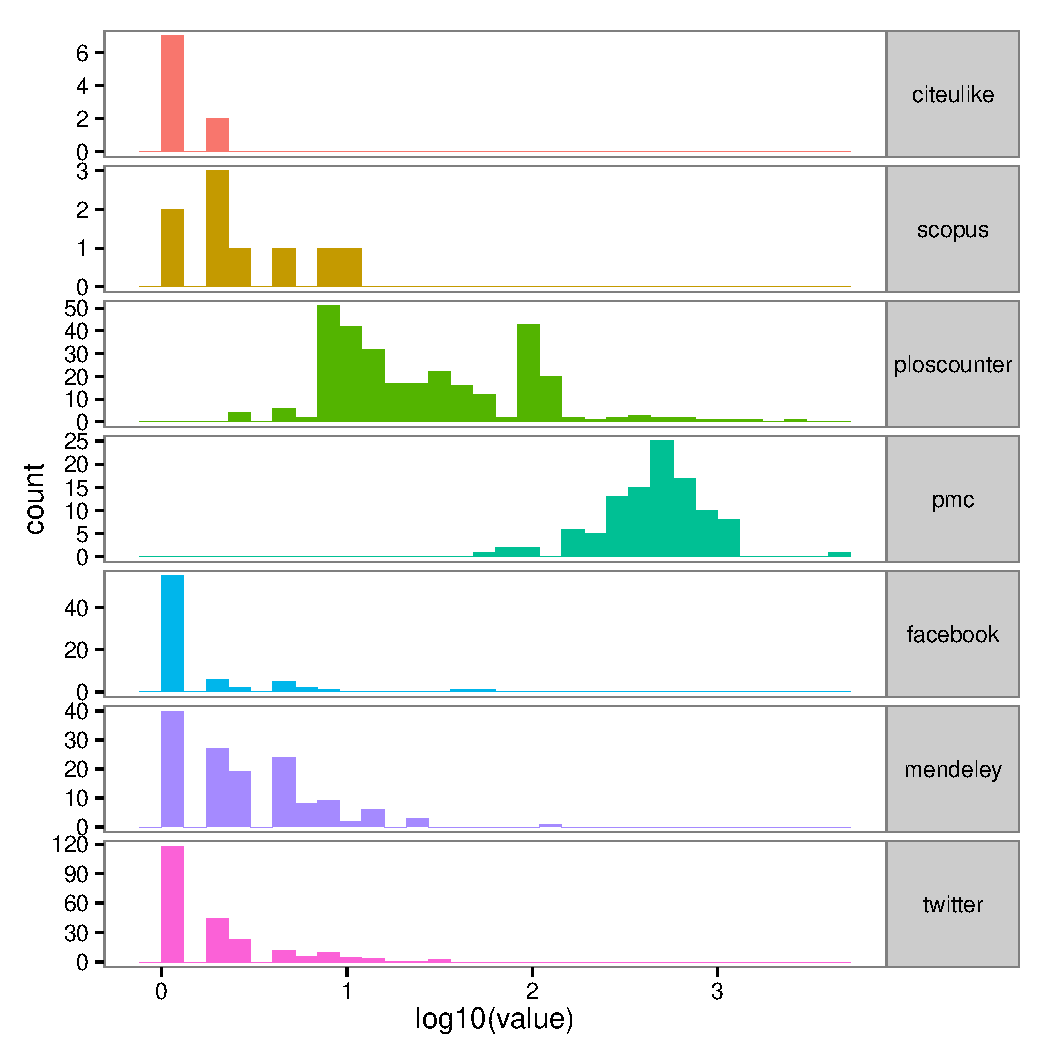
\includegraphics[width=0.7\textwidth]{figure/dataconst_plot.pdf}
%   \caption{Distribution of absolute differences in least and greatest value of each of seven different altmetrics on a set of 308 DOIs from Altmetric, ImpactStory, and PLoS ALM. Values were log10 transformed to improve comprehension.} % caption line
% \end{figure}

\begin{knitrout}
\definecolor{shadecolor}{rgb}{0.969, 0.969, 0.969}\color{fgcolor}\begin{figure}[]


{\centering 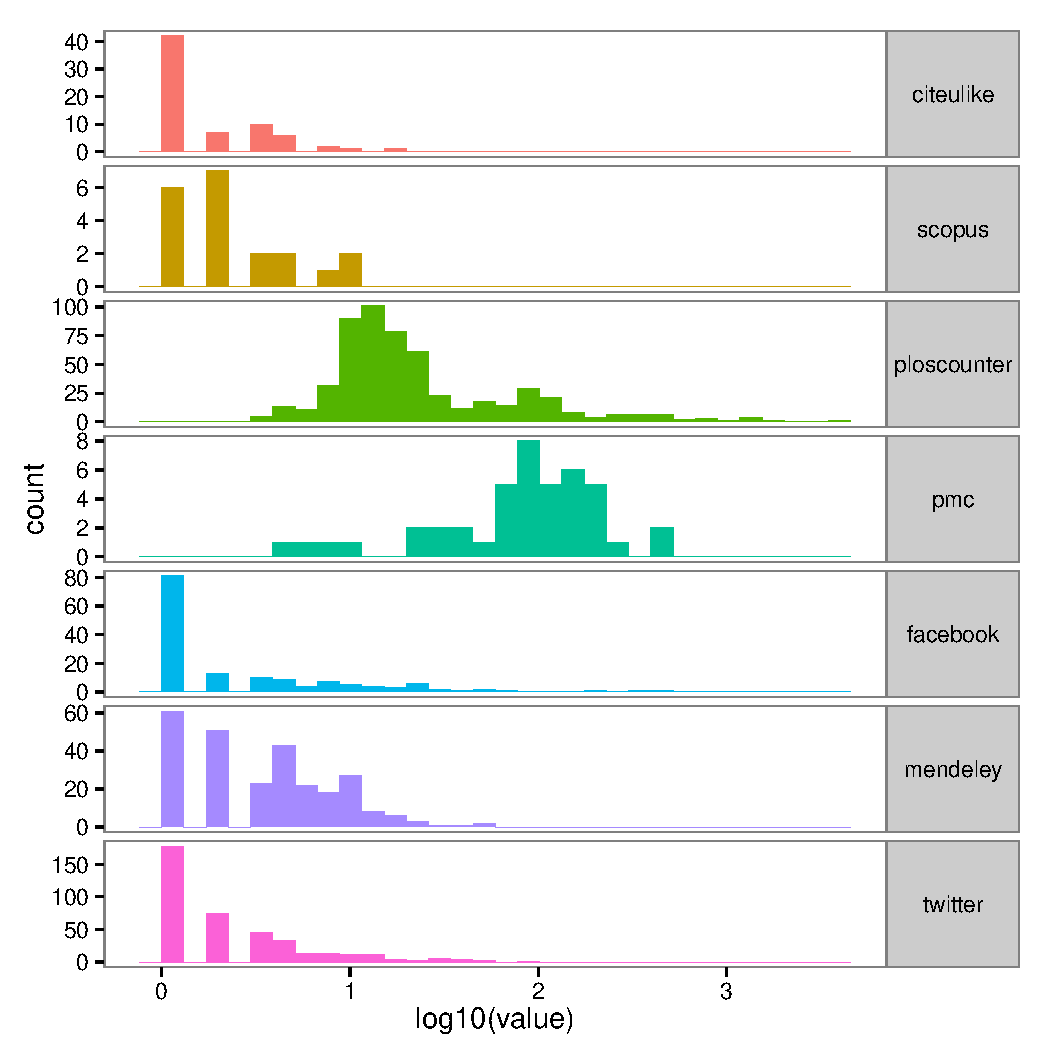
\includegraphics[width=.7\linewidth]{figure/dataconst_plot1} 

}

\caption[Distribution of absolute differences in least and greatest value of each of seven different altmetrics on a set of 565 DOIs from Altmetric, ImpactStory, and PLoS ALM]{Distribution of absolute differences in least and greatest value of each of seven different altmetrics on a set of 565 DOIs from Altmetric, ImpactStory, and PLoS ALM. Values were log10 transformed to improve visual comprehension.\label{fig:dataconst_plot1}}
\end{figure}


\end{knitrout}


What are some possible reasons why similar metrics differ across providers? Numbers could differ for a number of reasons. First, data could be collected from different middle-men. For example, Twitter data is notorious for not being persistent. Thus, you either have to query the Twitter firehose constantly and store data, or go through a company like Topsy (they collect twitter data and charge customers for access; http://topsy.com/) to collect tweets. Whereas ImpactStory collects tweets from Topsy, PLoS ALM and Altmetric collect tweets with an unknown method. Different intermediary data sources could lead to different data. Second, data could be collected at different times. This could easily result in different data even if data are collected from the same source. This is especially obvious as ImpactStory collects some metrics via the PLoS ALM API, so those metrics that ImpactStory has from the PLoS ALM API should be the same as those that PLoS has. Fortunately, date is supplied in the returned data by three of the providers (PLoS ALM, ImpactStory, and Altmetric). Thus, I examined whether or not date could explain differences in metrics from the different providers. Figure 2 shows that there are definitely some large differences in values that could be due differences in date the data was collected, but this is not always the case (i.e., there are a lot of large difference values with very small difference in dates). 

\begin{knitrout}
\definecolor{shadecolor}{rgb}{0.969, 0.969, 0.969}\color{fgcolor}\begin{figure}[]


{\centering 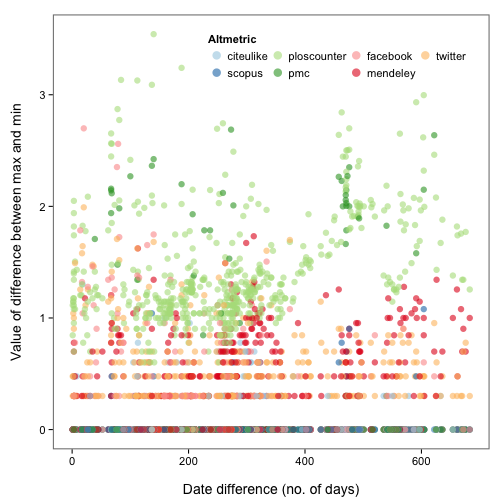
\includegraphics[width=.7\linewidth]{figure/dataconst_plot2} 

}

\caption[Distribution of absolute differences in least and greatest value of each of seven different altmetrics on a set of 565 DOIs from Altmetric, ImpactStory, and PLoS ALM]{Distribution of absolute differences in least and greatest value of each of seven different altmetrics on a set of 565 DOIs from Altmetric, ImpactStory, and PLoS ALM. Values were log10 transformed to improve visual comprehension.\label{fig:dataconst_plot2}}
\end{figure}


\end{knitrout}


That was a rough overview of hundreds of DOIs. What do the differences among providers look like in more detail? I used a set of 20 DOIs from the 565 above to show the value of each altmetric from each of the altmetrics providers for each of the 20 DOIs (see Fig. 3). Note that in some cases there is very close overlap in values for the same altmetric on the same DOI across providers, but in some cases the values are very different. 

\begin{knitrout}
\definecolor{shadecolor}{rgb}{0.969, 0.969, 0.969}\color{fgcolor}\begin{figure}[]


{\centering 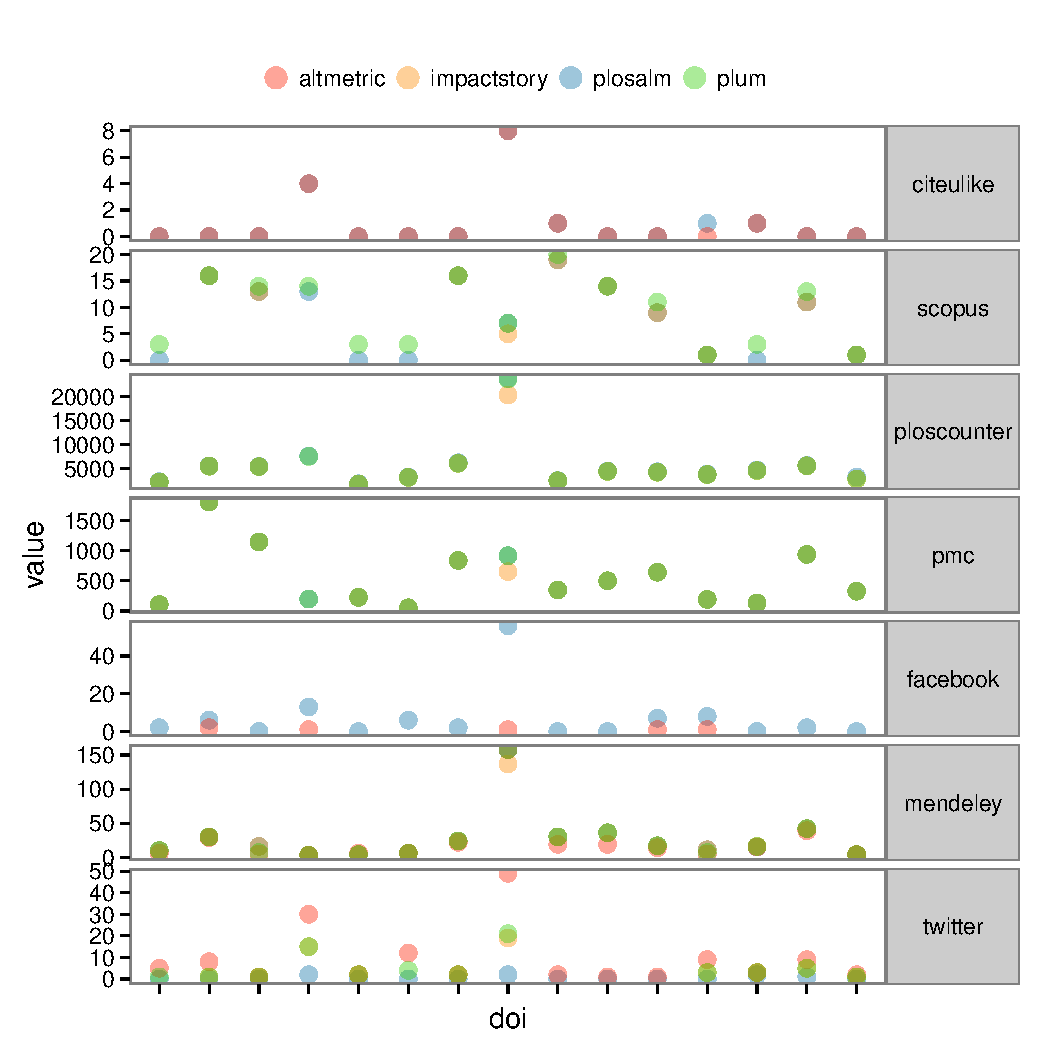
\includegraphics[width=.7\linewidth]{figure/dataconst2} 

}

\caption[A comparison of seven different altmetrics on a set of 20 DOIs from Altmetric, ImpactStory, and PLoS]{A comparison of seven different altmetrics on a set of 20 DOIs from Altmetric, ImpactStory, and PLoS. This demonstrates how altmetrics can be very similar across providers for some DOIs, but very dissimilar for others.\label{fig:dataconst2}}
\end{figure}


\end{knitrout}


An example giving what results look like may be instructive. Here is an example of calling the API of each the four providers to combine data from different sources, for the DOI \emph{10.1371/journal.pbio.1001118} \cite{arslan2011} (Table A2). There are many metrics that have exactly the same values among providers, though there are differences, which could be explained by the difference in the date data was collected. For example, PLoS ALM gives 3845 for combined PLoS views, while ImpactStory gives 3746 views. This is undoubtedly explained by the fact that PLoS ALM data was last updated on May 24, 2013, while ImpactStory's data was last updated on May 18, 2013. There are some oddities, however. For example, Altmetric gives nine tweets, while ImpactStory only gives three tweets. ImpactStory's data was updated more recently (May 18, 2013) than that of Altmetric (July 28, 2012), which suggests something different about the way tweets among the two providers are collected as updated date alone can not explain the difference. In fact, Table A1 shows that ImpactStory collects tweets from Topsy (\url{http://topsy.com/}), while Altmetric collects them with an unknown method, which leads to different data.

% latex table generated in R 2.15.3 by xtable 1.7-1 package
% Tue May 28 21:37:52 2013
\begin{table}[ht]
\centering
\caption{Example of combining results across three data providers on one DOI. Note that dates that data were last modified are the same for PLoS ALM and Altmetric, but different for ImpactStory. Missing values represent data that is not given by that provider.} 
\begin{tabular}{l|cccccccc}
  \hline
provider & citeulike & scopus & ploscounter & pmc & facebook & mendeley & twitter & date\_modified \\ 
  \hline
PLoS ALM & 1 & 1 & 3857 & 192 & 8 & 11 & 0 & 2013-05-28 \\ 
  Altmetric & 0 &  &  &  & 1 & 5 & 9 & 2012-07-28 \\ 
  ImpactStory &  & 1 & 3746 & 192 &  & 11 & 3 & 2013-05-18 \\ 
  PlumAnalytics &  & 1 & 3746 & 192 &  &  & 3 &  \\ 
   \hline
\end{tabular}
\end{table}



% \begin{figure}[!ht]
%   \centering
%   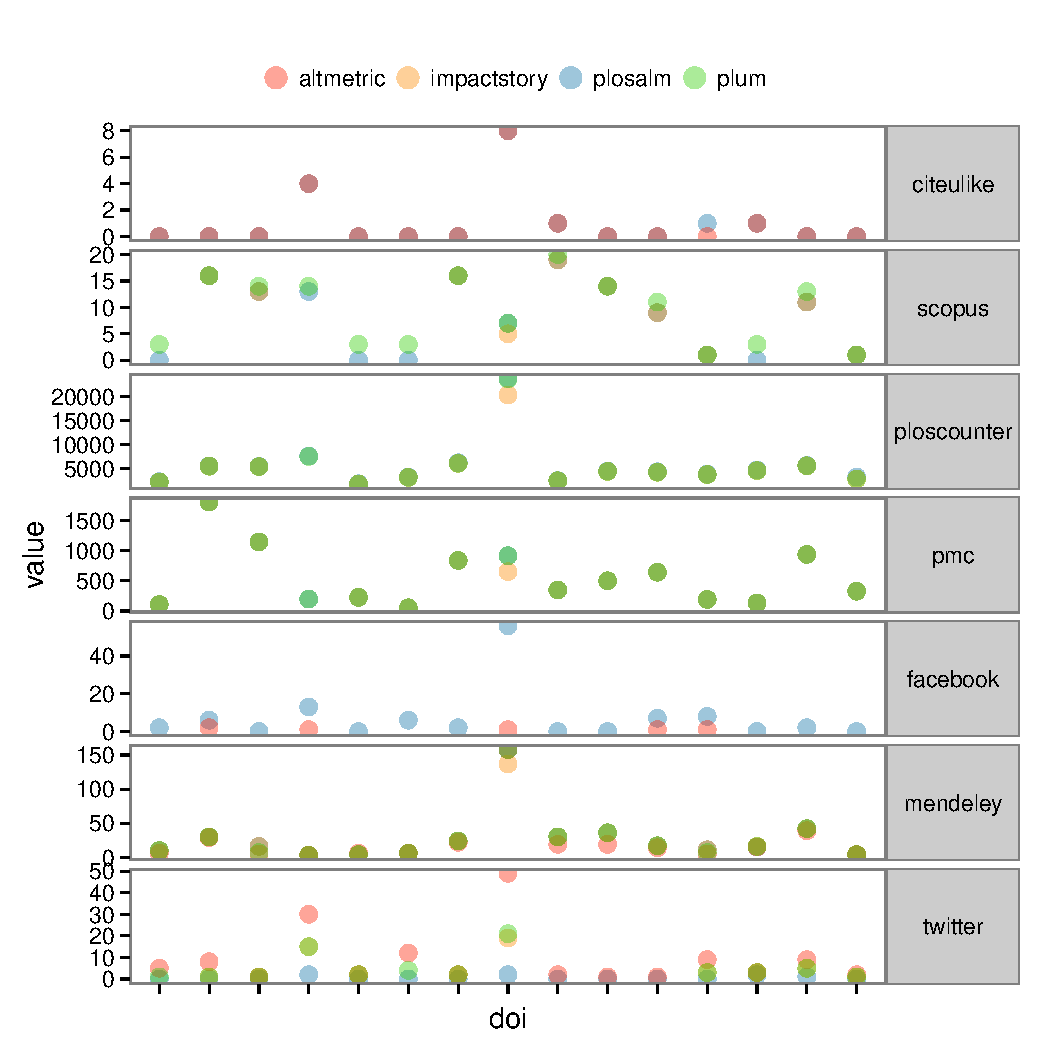
\includegraphics[width=0.7\textwidth]{figure/dataconst2.pdf}
%   \caption{A comparison of seven different altmetrics on a set of 20 DOIs from Altmetric, ImpactStory, and PLoS.} % caption line
% \end{figure}

The above findings on data consistency in fact suggest that altmetrics are inconsistent among providers of aggregate altmetrics. Casual users, and especially those conducting altmetrics research, should use caution when using altmetrics data.  

\subsection*{A crosswalk among providers}

As discussed above, when similar data sources are collected by altmetrics providers, ideally, there would be a way to go between, for example, data from Twitter for PLoS, ImpactStory, Altmetric, and PlumAnalytics. Each of the four providers of course has the right to collect metrics as needed for their purposes, but as altmetrics consumers, we should be able to compare data from the same source across providers. In Appendix Table A1, I provide a table to crosswalk metrics for the same data source among providers.

\section*{Altmetrics data provenance}

Altmetrics data comes from somewhere - tweets from Twitter, citations from Web of Science or Scopus, bookmarks from Citeulike, etc. Provenance is concerned with the origin of an object, the ability to trace where an object comes from in case there is any need to check or validate data. 

Why should we care about provenance in altmetrics?  First, in any research field we should prioritize research being verifiable. For this we need the underlying data. Second, in general, altmetrics are based on completely digital data. This means that all use of, research on, hiring decisions based on, and conclusions drawn from, altmetrics data should theoretically be traceable back to the original production of that data. This is somewhat unusual - most research fields are based on data collected at some point that can not be traced - but this should be possible in altmetrics. Second, a specific example will demonstrate the power of data provenance in altmetrics. Imagine if a research paper makes controversial claims using altmetrics data on a set of objects (e.g., scholarly papers). An independent researcher could theoretically drill down into the data collected for that paper, and gain further insight, and potentially dispute or add to the latter mentioned paper.

Data for the same altmetrics resource could be calculated in different ways and collected at different times for the same object. The four providers already provide the date the metrics were updated. However, there is little information available, via their APIs at least, regarding how data were collected, and what, if any, calculations were done on the data before providing the data. The altmetrics community overall would benefit from transparency in how data are collected. 

A good step in the right direction is that ImpactStory provides a field named \emph{provenance\_url} with each metric data source. For example, for a recent paper \cite{piwowar2007}, a GET call to the ImpactStory API returns many metrics, one of which is 10 bookmarks on Delicious. Importantly, they also return the field \emph{provenance\_url}, in this case \url{http://www.delicious.com/url/9df9c6e819aa21a0e81ff8c6f4a52029}, which takes you directly to the human readble page on Delicous from where the data was collected. This is important for researchers as ideally all of our research is replicable. A nice bit about digital data such as altmetrics is that we can trace back final altmetrics from providers such as ImpactStory to their original source.

The PLoS ALM API provides something less obvious with respect to provenance, a field called \emph{events\_url}, which for the same paper above \cite{piwowar2007} returns 82 bookmarks on Citeulike, and the human readable link to where the data was collected \url{http://www.citeulike.org/doi/10.1371/journal.pone.0000308}. 

Plum Analytics does something interesting with respect to provencance - in addition to the cononical URL, they collect alias URLs for each object that they collect metrics on. For example, for the DOI \emph{10.1371/journal.pone.0018657}, they collect many URLs that point to that paper. This makes sense as a digital product is inevitably going to end up living at more than one URL (the internete is a giant copying machine after all), so collecting URL aliases is a good step forward for altmetrics. It appears ImpactStory does this as well.

What is ideal with respect to data provenance? Is the link to where the original data was collected enough? Probably so, if no calculations were done on the original data before reaching users. However, some of the providers do give numbers which have been calculated. For example, ImpactStory puts some metrics into context by calculating a percentage relative to a reference set. Ideally, how this is done should be very clear, and verifiable. 

\section*{Putting altmetrics in context}

Raw altmetrics data can be number of tweets, or number of html views on a publishers website. What do these numbers mean? How does the paper or dataset I care about compare to others? ImpactStory gives context to their scores by classifying scores along two dimensions: audience (scholars or public) and type of engagement (view, discuss, save, cite, recommend). Users can then determine whether a product (paper, dataset, etc.) was highly viewed, discussed, saved, cited, or recommended, and by scientists, or by the public. This abstracts away many details; however, users can drill down to the underlying data via their API and web interface.  Altmetric uses a different approach. They provide context for only one metric, the altmetric score. This is a single aggregate metric, the calculation of which is not known. They do provide context for the altmetric score, including how it compares to a) all articles in the same journal, b) all articles in the same journal published within three weeks of the article, c) all articles in the Almetric database, and d) all articles in the Almetric database published within three weeks of the article. Altmetric gives detailed context for some altmetrics, including Facebook, Twitter, and blogs (see e.g., \url{http://altmetric.com/details.php?citation_id=1270911}). PlumAnalytics do not combine altmetrics into a single score as does Almetric, but do bin similar types of altmetrics into captures, citations, social media, mentions, and usage (\url{http://www.plumanalytics.com/metrics.html}; though you can dive into the indivdiual altmetrics). 

One of the advantages of altmetrics is the fact that they measure many different things, important to different stakeholders (public, scholars, funders) \cite{x,y}. Thus, combining altmetrics into a single score defeats one of the advantages of altmetrics over the traditional measure of impact, journal impact factor, a single metric summarising data on citations. The single Altmetric score is at first appealing given its apparent simplicity. However, if altmetrics are to avoid the mistakes befallen on the Journal Impact Factor \cite{ploseditorial}, we should strive for meaningful altmetrics important to different stakeholders, that retain their context (Tweets vs. citations). 

A specific example highlights the importance of context. A recent paper of much interest titled \emph{Glass shape influences consumption rate for alcoholic beverages} \cite{attwood2012} on the date of writing has an Altmetric score of ~316. This score is compared relative to the same journal (PLoS One), and all journals at different points in time. Other altmetrics are reported but are not given any context. ImpactStory reports no single score, gives raw altmetrics data and gives context. For example, ImpactStory reports that there are 149 tweets that mentioned the paper, and this number of tweets puts the paper 97th-100th percentile of all Web of Science indexed articles that year (2012). This context for tweets about an article is more informative than knowing that the paper has an Altmetric score of 316 - people should know the context for what audience tweets represent, and number of tweets relative to a reference set gives a bit of information on the impact of the paper relative to others. Of course not all journals are indexed by Web of Science, and the important reference set for one person (e.g., papers in journals in their specific field) may be different from another (e.g., papers for colleagues at their university or department). 

There is still work to with respect to context. Future work should consider further dimensions of context. For example, perhaps users should be able to decide how to put their metrics into context - instead of getting raw values and values relative to a pre-chosen reference set, users could choose what reference they want to use for their specific purpose. In addition, but much harder to achieve, is sentiment, or the meaning of the mention. That is, was a tweet or citation about a paper mentioned in a negative or positive light?

\section*{Historical context}

Researchers asking questions about altmetrics could ask more questions specifically dealing with time if historical altmetrics data were available. PLoS provides historical altmetrics data on some of their metrics (except in case of licenses, e.g., Web of Science, Scopus), while Altmetric provides only historical data on their Altmetric score (see below section \emph{Putting altmetrics in context}), and ImpactStory and Plum Analytics do not provide historical data. The data returned, for example, for number of tweets for an article from ImpactStory, Altmetric, or Plum Analytics is a cumulative sum of the tweets mentioning that article. What were the number of tweets mentioning the article one month ago, six months ago, one year ago? It is a great feature of PLoS ALM that you can get historical altmetrics data, but these data are only available for PLoS articles. The altmetrics community would benefit greatly from storing and making available historical almetrics data. Historical data, especially as more products are tracked, will become expensive to store, so perhaps won't be emphasized by altmetrics providers. In addition, a technical barrier comes in to play in that pushing a lot of data via an API call can get very time consuming. 

% \section*{Relavance of altmetrics}
% The internet has facilitated the existence of altmetrics, as measures of impact are all around us, and many are now machine readable. However, which altmetrics are % relavant? More importantly, which altmetrics are relavant to the community you care about? XXXX. [NOT SURE IT MAKES SENSE TO KEEP THIS SECTION???]

%\section*{Open altmetrics}

%The Journal Impact Factor (JIF), based on citation counts, the predecessor in a way to altmetrics, is a closed metric, calculated by one company, the calculation of which is unknown \cite{rossner2007show}. Given that the altmetrics movement is just at its begining, it has the chance to be a more transparent endeavour. There are a number of companies and apps appearing to provide services on top of altmetrics, some of which to create profits need to protect data outputs and the details of their operations.  Regardless, I think the altmetrics community can and should provide a level of transparency and openness that will allow research on, and use of, altmetrics. Openness in altmetrics can only be good for the science. If altmetrics are transparent, conclusions from papers, hiring decisions, and more can be verified by third parties. In addition, transparent altmetrics are less likely to be gamed, as they JIF has been gamed \cite{arnold2011}. Some good steps have been made to open altmetrics by altmetrics providers themselves. For example, many conferences and meetings have occurred where altmetrics providers and other interested parties hash out issues. 

%Another issue to consider in open altmetrics are the primary altmetrics sources. The difference between Twitter and App.net is a good example. Twitter makes money off advertisements and having a relatively closed system (\url{http://techonomy.com/2012/08/video-jack-dorsey-on-twitters-business-model/}). A better option, with similar data, would be App.net. App.net has a much smaller set of users relative to Twitter - however, App.net's business model is to charge users to use the service, but make the data very open. Twitter makes more money from closing down data, whereas App.net makes more money from opening up their data. There is currently a heavy dependence on Twitter in the altmetrics community. Perhaps we should think about building the scientific community on App.net where openness can thrive. 

\section*{Technical barriers to use}

Some altmetrics users may only require basic uses of altmetrics, like including altmetrics on their CV's \cite{piwowar2013power} to show the various impacts of their research. Some may want to go deeper, and perhaps collect altmetrics at finer time scales, or with more detailed data, than are given by altmetrics aggregate providers. What are the barriers to getting more detailed altmetrics data? 

Diving deeper into altmetrics means considering whether one can access data, whether the data source is machine readable, and how easy the data is to retrieve and manipulate once retrieved. 

\begin{itemize}
  \item \emph{Data access} Many altmetrics sources are accessible as the data providers have open, or at least partly open, APIs (e.g., Crossref, PLoS). Other data sources can provide problems. For example, you can only get tweets from Twitter for the past 30 days, after which point you have to pay for a service that caches historical Twitter data (e.g, Topsy). Others are totally inaccessable (e.g., Google Scholar citations). 
  \item \emph{Machine readable} Ideally, altmetrics are provided through an API. However, some metrics of interest may only be in PDFs, spreadsheets, or html, which can not be easily consumed and mashed up. For these metrics, the user should seek out aggregators such as those discussed in this paper to do the heavy lifting. Alternatively, technically savy researchers could write their own code, or leverage tools such as ScraperWiki \url{https://scraperwiki.com/}. 
  \item \emph{Ease of use} Fortunately, many libraries, or extensions, exist for a number of programming languages relavant to scholars (Python, R), which deal with interacting with altmetricsc data (e.g., Figshare API libraries \cite{figshare}, Twitter API libraries \cite{twitter}). See Table 1 for links to libraries for aggregate providers. These libraries take care of the data collection and transform data to user friendly objects, allowing users to do the real work of analysis and inference.
\end{itemize}

%Last, authentication can be a barrier to use in that if a user has to take extra step of authenticating, they may not bother. There are a variety of possible authentication methods, some of which include: a) no authentication, b) username and password pair, c) API key, and d) OAuth (including OAuth1 and OAuth2) (Table 1). These different options make sense in different use cases. The first, no authentication, used by PLoS, makes sense when an API is first released and testers are needed to get feedback. A benefit of an API with no authentication is the barrier to entry is lower. That is, if you don't have to ask a user to register to get an API key they are more likely to use the API. The second and third options, username/password pair and API key are relatively similar; API keys are used by both ImpactStory and Altmetric (Table 1). The last option, OAuth, is not used by any of the altmetrics providers. This authentication method is however used by many API providers. From the viewpoint of a consumer in a desktop scripting language, OAuth can be painful. What works better for scripting languages are the first three options.  

\section*{Conclusion}

Altmetrics measure the impact of scholarly articles and other products (e.g., datasets, presentations). These measures of scholarly impact are quickly gaining ground as evidenced by the four companies aggregating and providing altmetrics (see Table 1). In any field growing pains are inevitable - altmetrics as a field is quite young, and therefore has some issues to work out. I have shown in this paper that while the four providers aren't doing anything wrong or intentionally misleading, altmetrics users should think about a variety of issues when using altmetrics data: consistency, provenance, and context. Altmetrics providers collect data at different times, and from different sources; combining data across providers should be done with care. Altmetrics is special in the sense that all data is digital. Thus, there is no reason we shouldn't be able to track all altmetrics data to their sources. This will not only provide additional insight to scholarly impact, but provide a way to verify results and conclusions made regarding altmetrics. 

As altmetrics grow in use and popularity, researchers will ask more questions about altmetrics. In addition, it is hard to predict what people will want to do with altmetrics data in the future. Since we are in the early stages of the field of altmetrics, we have the chance to steer the altmetrics ship in the right direction. I hope the points covered in this paper provide fodder almetrics providers and users to consider.

\section*{Acknowledgments}

I thank Martin Fenner for inviting me to write a paper in this special issue on altmetrics, and for helpful feedback from Carl Boettiger and Karthik Ram on earlier versions of this manuscript.
  
\section*{References}
\bibliography{refs}

\section*{Appendix A. Crosswalk among providers.}

The following Table A1 provides a crosswalk between altmetrics data collected by the three data providers. Note that these variables relate to one another across providers, but the data may be collected differently, and so for example, altmetrics collected for Twitter may differ between PLoS, ImpactStory and Altmetric. Where data sources are shared among at least two providers, I used only those fields that would give the same data if data were collected on the same date and all other things being equal. For example, PLoS ALM's field \emph{pubmed} is equivalent to ImpactStory's \emph{pubmed:pmc\_citations} field.

\begin{table}[!ht]
\begin{threeparttable}[b]
\caption{Data sources used in taxize, tasks available, and links to them}
\begin{tabular}{|B|B|B|B|D}
\hline
\headcol Data source & PLoS\tnote{a} & ImpactStory\tnote{b} & Altmetric\tnote{c} & PlumAnalytics\tnote{d} \\
\hline
Biod & biod & No & No \\
\rowcol Connotea & connotea & No & No & No \\
Bloglines & bloglines & No & No & No \\
\rowcol Nature blogs & nature & No & No & No\\
Postgenomic & postgenomic & No & No & No \\
\rowcol Researchblogging & researchblogging & No & No & ResearchBlogging \\
WebOfScience citations & webofscience & No & No & No \\
\rowcol Dryad & No & dryad:total\_downloads package\_views & No & Views, downloads \\
Figshare & No & figshare:views shares downloads & No & Recommendations, downloads, views \\
\rowcol Github & No & github:forks stars & No & Collaborators, downloads, followers, forks, watches, gists \\
PLoS Search & No & plossearch:mentions & No & No \\
\rowcol Slideshare & No & slideshare:favorites views comments downloads & No & Downloads, favorites, comments \\
Google+ & No & No & cited by gplus count & No. +1's \\
\rowcol MSM & No & No & cited by msm count & No \\
News articles & No & No & Yes & Yes \\
\rowcol Reddit & No & No & cited by rdts count & Comments, upvotes-downvotes \\
Citeulike & citeulike & citeulike:bookmarks & No & Citeulike \\
\rowcol Crossref & crossref & plosalm:crossref\tnote{e} & No & No \\
PLoS ALM & counter(pdf\_views + html\_views)\tnote{f} & plosalm(html\_views, pdf\_views) & No & Views of abstract, figures, full text, html, pdf, supporting data \\
\rowcol PMC & pmc & plosalm:pmc\_full-text + pmc\_pdf\tnote{g} & No & No \\
PubMed & pubmed & pubmed:pmc\_citations\tnote{h} & No & Pumbed \\
\rowcol Scienceseeker & scienceseeker & scienceseeker:blog\_posts & No & ScienceSeeker \\
Scopus citations & scopus & plosalm:scopus\tnote{i} & No & Scopus \\
\rowcol Wikipedia & wikipedia & wikipedia:mentions & No & Wikipedia \\
Delicious & No & delicious:bookmarks & cited by delicious count & Delicious \\
\rowcol Facebook & facebook\_shares & facebook:shares\tnote{j} & cited by fbwalls count & Facebook clicks, comments, likes \\
Mendeley readers & mendeley shares & mendeley readers\tnote{k} & mendeley readers & Mendeley readers, groups \\
\rowcol Twitter & twitter & topsy:tweets\tnote{l} & cited by tweeters count & Topsy tweets \\
\hline
\end{tabular}
% \begin{tablenotes}
%     \item[a] These are the exact names for each data source in the PLos ALM API. For example: \url{http://alm.plos.org/api/v3/articles?ids=10.1371/journal.pone.0018657&source=twitter}.
%     \item[b] You can not request a specific source from the ImpactStory API, so these are the names of the fields in the returned json. For example, see the json from this call: \url{http://api.impactstory.org/v1/item/doi/10.1371/journal.pone.0018657?key=YOURAPIKEY}.
%     \item[c] You can not request a specific source from the Altmetric API, so these are the names of the fields in the returned json. For example, see the json from this call: \url{http://api.altmetric.com/v1/doi/10.1371/journal.pbio.0018657?key=YOURAPIKEY}.
%     \item[d] Some of these names are the exact names returned in an API call; others are not.
%     \item[e] Collected from the PLoS ALM API. 
%     \item[f] PLoS ALM also provides xml\_views. 
%     \item[g] Collected from the PLoS ALM API. Other PMC data fields collected from PLoS ALM (pmc\_abstract, pmc\_supp-data, pmc\_figure, pmc\_unique-ip) and from PubMed (suppdata\_views, figure\_views, unique\_ip\_views, pdf\_downloads, abstract\_views, fulltext\_views).
%     \item[h] Should be equivalent to plosalm:pubmed\_central. ImpactStory also collects pubmed:pmc\_citations\_reviews f1000 pmc\_citations\_editorials.
%     \item[i] Collected from the PLoS ALM API. Scopus citations also collected from Scopus itself, in the field scopus:citations.
%     \item[j] ImpactStory also collects Facebook clicks, comments, and likes. 
%     \item[k] ImpactStory also collects Mendeley readers by discipline, number of groups that have added the article, percent of readers by country, and percent of readers by career\_stage. 
%     \item[l] ImpactStory also collects the number of influential\_tweets from Topsy.
% \end{tablenotes}
\end{threeparttable}
\end{table}

Footnotes from Table A1.

\begin{itemize}
    \item[a] These are the exact names for each data source in the PLos ALM API. For example: \url{http://alm.plos.org/api/v3/articles?ids=10.1371/journal.pone.0018657&source=twitter}.
    \item[b] You can not request a specific source from the ImpactStory API, so these are the names of the fields in the returned json. For example, see the json from this call: \url{http://api.impactstory.org/v1/item/doi/10.1371/journal.pone.0018657?key=YOURAPIKEY}.
    \item[c] You can not request a specific source from the Altmetric API, so these are the names of the fields in the returned json. For example, see the json from this call: \url{http://api.altmetric.com/v1/doi/10.1371/journal.pbio.0018657?key=YOURAPIKEY}.
    \item[d] Some of these names are the exact names returned in an API call; others are not.
    \item[e] Collected from the PLoS ALM API. 
    \item[f] PLoS ALM also provides xml\_views. 
    \item[g] Collected from the PLoS ALM API. Other PMC data fields collected from PLoS ALM (pmc\_abstract, pmc\_supp-data, pmc\_figure, pmc\_unique-ip) and from PubMed (suppdata\_views, figure\_views, unique\_ip\_views, pdf\_downloads, abstract\_views, fulltext\_views).
    \item[h] Should be equivalent to plosalm:pubmed\_central. ImpactStory also collects pubmed:pmc\_citations\_reviews f1000 pmc\_citations\_editorials.
    \item[i] Collected from the PLoS ALM API. Scopus citations also collected from Scopus itself, in the field scopus:citations.
    \item[j] ImpactStory also collects Facebook clicks, comments, and likes. 
    \item[k] ImpactStory also collects Mendeley readers by discipline, number of groups that have added the article, percent of readers by country, and percent of readers by career\_stage. 
    \item[l] ImpactStory also collects the number of influential\_tweets from Topsy.
\end{itemize}

\end{document}
